\uuid{Y0PJ}
\exo7id{5199}
\titre{exo7 5199}
\auteur{rouget}
\organisation{exo7}
\datecreate{2010-06-30}
\isIndication{false}
\isCorrection{true}
\chapitre{Géométrie affine dans le plan et dans l'espace}
\sousChapitre{Géométrie affine dans le plan et dans l'espace}
\module{Géométrie}
\niveau{L2}
\difficulte{}

\contenu{
\texte{
Soit $(E)$ l'ensemble d'équation cartésienne $2x^2+5xy+3y^2-3x-2y-5=0$. Montrer que $(E)$ est une réunion de deux droites. Déterminer l'aire du parallélogramme formé par ces deux droites et les parallèles à ces deux droites passant par $O$.
}
\reponse{
Soit $(x,y)\in\Rr^2$.

\begin{align*}
2x^2+5xy+3y^2-3x-2y-5&=2x^2+x(5y-3)+3y^2-2y-5=2(x+\frac{1}{4}(5y-3))^2-\frac{1}{8}(5y-3)^2+3y^2-2y-5\\
 &=\frac{1}{8}(4x+5y-3)^2-\frac{1}{8}y^2+\frac{14}{8}y-\frac{49}{8}\\
 &=\frac{1}{8}[(4x+5y-3)^2-(y^2-14y+49)]=\frac{1}{8}[(4x+5y-3)^2-(y-7)^2]\\
 &=\frac{1}{8}(4x+4y+4)(4x+6y-10)=(x+y+1)(2x+3y-5)
\end{align*}

Par suite,

$$\forall(x,y)\in\Rr^2,\;2x^2+5xy+3y^2-3x-2y-5=0\Leftrightarrow(x+y+1=0\;\mbox{ou}\;2x+3y-5=0.$$

$(E)$ est la réunion de la droite $(D_1)$ d'équation $x+y+1=0$ et de la droite $(D_2)$ d'équation $2x+3y-5=0$.

$$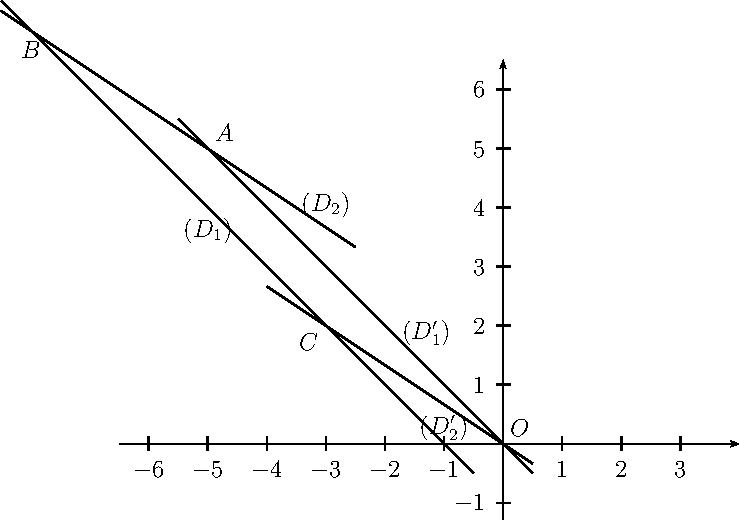
\includegraphics{../images/pdf/Y0PJ-1.pdf}$$

La parallèle à $(D_1)$ passant par $O$ est la droite $(D_1')$ d'équation $x+y=0$ et la parallèle à $(D_2)$ passant par $O$ est la droite $(D_2')$ d'équation $2x+3y=0$. Ces droites se coupent en les quatre points $O(0,0)$, $A(-5,5)$, $B(-8,7)$ et $C(-3,2)$. L'aire de ce parallélogramme vaut $\left|\mbox{det}(\overrightarrow{OA},\overrightarrow{OC})\right|=5$.
}
}
